
\documentclass[UTF8]{article}
\usepackage{xeCJK}
\usepackage{amsmath,amssymb}
\begin{document}


  

   \chapter{Operating system organization}   
    \label{CH:FIRST}     

操作系统的一个关键要求是同时支持多个活动。例如,使用 Chapter~    \ref{CH:UNIX}    中描述的系统调用接口,进程可以启动新进程:
    \lstinline{fork}    。操作系统必须
    \indextext{time-share}    这些进程中的计算机资源。例如,即使进程数量多于硬件 CPU 数量,操作系统也必须确保所有进程都有机会执行。操作系统还必须安排
 进程之间的    \indextext{isolation}   。也就是说,如果一个进程有错误并且发生故障,它不应该影响不依赖于有错误的进程的进程。然而,完全隔离太强了,因为进程应该可以有意地交互;管道就是一个例子。因此操作系统必须满足三个要求:复用、隔离和交互。  

本章概述了如何组织操作系统来实现这三个要求。事实证明,有很多方法可以做到这一点,但本文重点关注以    \indextext{monolithic kernel}    为中心的主流设计,许多 Unix 操作系统都使用它。本章还概述了 xv6 进程(xv6 中的隔离单元),以及 xv6 启动时第一个进程的创建。  

Xv6 在    \indextext{multi-core}       \footnote{本文中的“多核”是指共享内存但并行执行的多个 CPU,每个 CPU 都有自己的一组寄存器。本文有时使用术语
    \indextext{multiprocessor}    是多核的同义词,但多处理器也可以更具体地指具有多个不同处理器芯片的计算机。  }    RISC-V 微处理器上运行,其许多低级功能(例如,其流程实现)特定于 RISC-V。 RISC-V是64位CPU,xv6是用“LP64”C编写的,这意味着C编程语言中的long(L)和指针(P)是64位,但int是32位。本书假设读者已经在某些架构上完成了一些机器级编程,并将在出现时介绍 RISC-V 特定的想法。 RISC-V 的有用参考是“RISC-V 阅读器:开放架构图集”~    \cite{riscv}   。用户级 ISA~    \cite{riscv:user}    和特权架构~    \cite{riscv:priv}    是官方规范。  

完整计算机中的 CPU 周围环绕着支持硬件,其中大部分以 I/O 接口的形式存在。 Xv6 是为 qemu 的“-machine virt”选项模拟的支持硬件而编写的。这包括 RAM、包含启动代码的 ROM、与用户键盘/屏幕的串行连接以及用于存储的磁盘。
    \section{抽象物理资源  }     

当遇到操作系统时,人们可能会问的第一个问题是为什么要有它?也就是说,可以将图 ~    \ref{fig:api}    中的系统调用实现为一个库,应用程序可以与该库链接。在这个计划中,每个应用程序甚至可以拥有自己的适合其需求的库。应用程序可以直接与硬件资源交互,并以最适合应用程序的方式使用这些资源(例如,实现高或可预测的性能)。一些嵌入式设备或实时系统的操作系统就是以这种方式组织的。  

这种库方法的缺点是,如果有多个应用程序正在运行,则这些应用程序必须表现良好。例如,每个应用程序必须定期放弃CPU,以便其他应用程序可以运行。如果所有应用程序相互信任并且没有错误,那么这种协作分时方案可能是可行的。对于应用程序来说,更常见的是彼此不信任并且存在错误,因此人们通常需要比协作方案提供的更强的隔离。  

为了实现强隔离,禁止应用程序直接访问敏感硬件资源,并将资源抽象为服务,会很有帮助。例如,Unix 应用程序仅通过文件系统的
    \lstinline{open}    ,
    \lstinline{read}    ,
    \lstinline{write}    和
    \lstinline{close}   系统调用,而不是直接读写磁盘。这为应用程序提供了路径名的便利,并且允许操作系统(作为接口的实现者)管理磁盘。即使隔离不是一个问题,有意交互(或只是希望不妨碍彼此)的程序也可能会发现文件系统是比直接使用磁盘更方便的抽象。  

类似地,Unix在进程之间透明地切换硬件CPU,根据需要保存和恢复寄存器状态,这样应用程序就不必担心时间共享。即使某些应用程序处于无限循环中,这种透明度也允许操作系统共享 CPU。  

另一个例子,Unix 进程使用
    \lstinline{exec}    来构建它们的内存映像,而不是直接与物理内存交互。这允许操作系统决定将进程放置在内存中的位置;如果内存紧张,操作系统甚至可能将某些进程的数据存储在磁盘上。
    \lstinline{exec}   还为用户提供了方便的文件系统来存储可执行程序映像。  

Unix 进程之间的许多交互形式都是通过文件描述符发生的。文件描述符不仅抽象了许多细节(例如,管道或文件中的数据存储位置),而且还以简化交互的方式进行定义。例如,如果管道中的一个应用程序失败,内核将为管道中的下一个进程生成文件结束信号。  

图~   \ref{fig:api}   中的系统调用接口经过精心设计,既为程序员提供了便利,又提供了强隔离的可能性。 Unix 接口并不是抽象资源的唯一方法,但它已被证明是一个非常好的方法。
    \section{用户模式、管理员模式和系统调用  }     

强隔离需要应用程序和操作系统之间有硬边界。如果应用程序出错,我们不希望操作系统失败或其他应用程序失败。相反,操作系统应该能够清理失败的应用程序并继续运行其他应用程序。为了实现强隔离,操作系统必须安排应用程序不能修改(甚至读取)操作系统的数据结构和指令,并且应用程序不能访问其他进程的内存。  

CPU为强隔离提供硬件支持。例如,RISC-V具有三种CPU执行指令的模式:
    \indextext{machine mode}    ,
    \indextext{supervisor mode}    和
    \indextext{user mode}    。在机器模式下执行的指令具有完全特权; CPU 以机器模式启动。机器模式主要用于配置计算机。 Xv6 在机器模式下执行几行,然后更改为管理模式。  

在管理模式下,CPU 可以执行
    \indextext{privileged instructions}    :例如,启用和禁用中断、读取和写入保存页表地址的寄存器等。如果用户模式下的应用程序尝试执行特权指令,则CPU不会执行该指令,而是切换到管理程序模式,以便主管模式代码可以终止应用程序,因为它做了一些不应该做的事情。第〜   \ref{CH:UNIX}   中的图〜   \ref{fig:os}   说明了这种组织。应用程序只能执行用户模式指令(例如,添加数字等),并且据说运行在
    \indextext{user space}   ,而管理模式下的软件也可以执行特权指令,据说运行在
    \indextext{kernel space}    。运行在内核空间(或管理模式)的软件称为
    \indextext{kernel}    。  

想要调用内核函数的应用程序(例如
 xv6 中的    \lstinline{read}    系统调用必须转换到内核;应用程序不能直接调用内核函数。 CPU 提供了一种特殊的指令,可以将 CPU 从用户模式切换到管理模式,并在内核指定的入口点进入内核。 (RISC-V 提供
    \indexcode{ecall}    指令用于此目的。)一旦 CPU 切换到管理模式,内核就可以验证系统调用的参数(例如,检查传递给系统调用的地址是否是应用程序内存的一部分),决定应用程序是否允许执行请求的操作(例如,检查应用程序是否允许写入指定的文件),然后拒绝或执行它。内核控制转换到管理模式的入口点非常重要;例如,如果应用程序可以决定内核入口点,则恶意应用程序可以在跳过参数验证的点进入内核。
    \section{内核组织  }     

一个关键的设计问题是操作系统的哪一部分应该在管理模式下运行。一种可能性是整个操作系统驻留在内核中,以便所有系统调用的实现都在管理程序模式下运行。这个组织被称为
    \indextext{monolithic kernel}    。  

在这个组织中,整个操作系统以完全的硬件权限运行。这种组织很方便,因为操作系统设计者不必决定操作系统的哪一部分不需要完整的硬件权限。此外,操作系统的不同部分更容易协作。例如,操作系统可能具有可由文件系统和虚拟内存系统共享的缓冲区高速缓存。  

整体组织的缺点是操作系统不同部分之间的接口通常很复杂(正如我们将在本文的其余部分中看到的),因此操作系统开发人员很容易犯错误。在单片内核中,错误是致命的,因为管理模式下的错误通常会导致内核失败。如果内核出现故障,计算机就会停止工作,因此所有应用程序也会失败。计算机必须重新启动才能重新启动。  

为了降低内核出错的风险,操作系统设计者可以最大限度地减少在管理模式下运行的操作系统代码量,并在用户模式下执行操作系统的大部分代码。这个内核组织称为
    \indextext{microkernel}    。  

   \begin{figure}[t]
\center
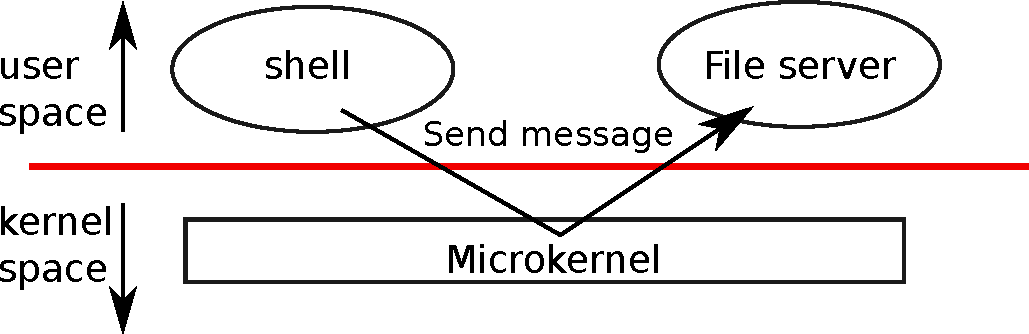
\includegraphics[scale=0.5]{fig/mkernel.pdf}
\caption{带有文件系统服务器的微内核  }
\label{fig:mkernel}
\end{figure}     

图~    \ref{fig:mkernel}    说明了这种微内核设计。在图中,文件系统作为用户级进程运行。作为进程运行的操作系统服务称为服务器。为了允许应用程序与文件服务器交互,内核提供了进程间通信机制,将消息从一个用户模式进程发送到另一个用户模式进程。例如,如果像 shell 这样的应用程序想要读取或写入文件,它会向文件服务器发送一条消息并等待响应。  

在微内核中,内核接口由一些低级函数组成,用于启动应用程序、发送消息、访问设备硬件等。这种组织使内核相对简单,因为大多数操作系统驻留在用户级服务器中。  

在现实世界中,整体内核和微内核都很流行。许多 Unix 内核都是单一的。例如,Linux 具有整体内核,尽管某些操作系统功能作为用户级服务器运行(例如窗口系统)。 Linux 为操作系统密集型应用程序提供了高性能,部分原因是内核的子系统可以紧密集成。  

Minix、L4 和 QNX 等操作系统被组织为带有服务器的微内核,并且在嵌入式设置中得到了广泛部署。 L4 的变体 seL4 足够小,已经过内存安全和其他安全属性的验证~    \cite{sel4}    。  

关于哪个组织更好,操作系统开发人员之间存在很多争论,并且没有任何确凿的证据。此外,它很大程度上取决于“更好”的含义:更快的性能、更小的代码大小、内核的可靠性、整个操作系统的可靠性(包括用户级服务)等。  

还有一些实际考虑因素可能比哪个组织的问题更重要。一些操作系统具有微内核,但出于性能原因在内核空间中运行一些用户级服务。一些操作系统具有整体内核,因为它们就是这样开始的,并且几乎没有动力转向纯粹的微内核组织,因为新功能可能比重写现有操作系统以适应微内核设计更重要。  

从本书的角度来看,微内核和单片操作系统有许多共同的关键思想。它们实现系统调用、使用页表、处理中断、支持进程、使用锁进行并发控制、实现文件系统等。本书重点讨论这些核心思想。  

与大多数 Unix 操作系统一样,Xv6 是作为整体内核实现的。由此可见,xv6内核接口对应于操作系统接口,内核实现了完整的操作系统。由于 xv6 不提供很多服务,因此它的内核比某些微内核要小,但从概念上讲 xv6 是整体的。  

   \section{代码:xv6 组织  }     

   \begin{figure}[t]
\center
\begin{tabular}{l|l}
{\bf File} & {\bf Description}  \\ 
\midrulebio.c & Disk block cache for the file system.  \\ console.c & Connect to the user keyboard and screen.  \\ entry.S & Very first boot instructions.  \\ exec.c & exec() system call.  \\ file.c & File descriptor support.  \\ fs.c & File system.  \\ kalloc.c & Physical page allocator.  \\ kernelvec.S & Handle traps from kernel, and timer interrupts.  \\ log.c & File system logging and crash recovery.  \\ main.c & Control initialization of other modules during boot.  \\ pipe.c & Pipes.  \\ plic.c & RISC-V interrupt controller.  \\ printf.c & Formatted output to the console.  \\ proc.c & Processes and scheduling.  \\ sleeplock.c & Locks that yield the CPU.  \\ spinlock.c & Locks that don't yield the CPU.  \\ start.c & Early machine-mode boot code.  \\ string.c & C string and byte-array library.  \\ swtch.S & Thread switching.  \\ syscall.c & Dispatch system calls to handling function.  \\ sysfile.c & File-related system calls.  \\ sysproc.c & Process-related system calls.  \\ trampoline.S & Assembly code to switch between user and kernel.  \\ trap.c & C code to handle and return from traps and interrupts.  \\ uart.c & Serial-port console device driver.  \\ virtio\_disk.c & Disk device driver.  \\ vm.c & Manage page tables and address spaces.  \\ 
\end{tabular}
\caption{Xv6 内核源文件。  }
\label{fig:source}
\end{figure}     

xv6 内核源代码位于  {    \tt   内核/   }  子目录中。源代码被分成文件,遵循模块化的粗略概念;图~    \ref{fig:source}    列出了这些文件。模块间接口在    \lstinline{defs.h}       \fileref{kernel/defs.h}    中定义。
    \section{流程概览  }     

xv6 中的隔离单位(与其他 Unix 操作系统一样)是
    \indextext{process}    。进程抽象可以防止一个进程破坏或监视另一个进程的内存、CPU、文件描述符等。它还可以防止进程破坏内核本身,因此进程无法破坏内核的隔离机制。内核必须小心地实现进程抽象,因为有错误或恶意的应用程序可能会欺骗内核或硬件做一些坏事(例如,规避隔离)。内核用来实现进程的机制包括用户/管理程序模式标志、地址空间和线程的时间分片。  

为了帮助实施隔离,进程抽象为程序提供了它拥有自己的私有机器的错觉。进程为程序提供了看似私有的内存系统,或者
    \indextext{address space}    ,其他进程无法读取或写入。进程还为程序提供看似其自己的 CPU 来执行程序的指令。  

Xv6 使用页表(由硬件实现)为每个进程提供自己的地址空间。 RISC-V 页表转换(或“映射”)a
    \indextext{virtual address}   (RISC-V 指令操作的地址)到
    \indextext{physical address}   (CPU芯片发送到主存的地址)。  

   \begin{figure}[t]
\centering
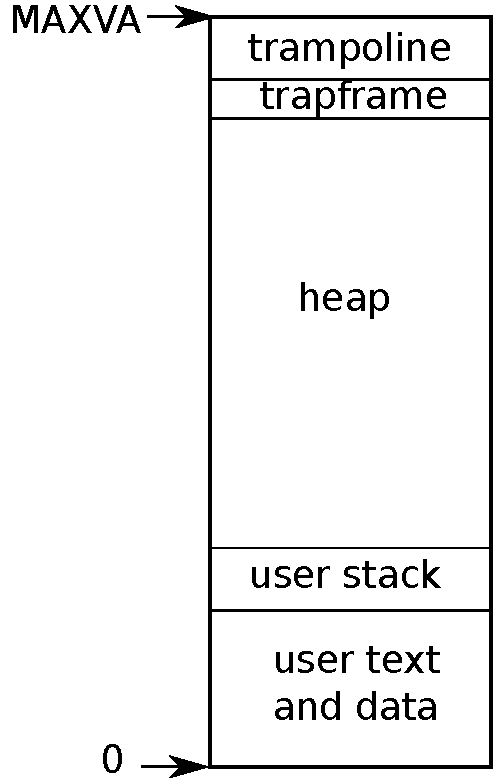
\includegraphics[scale=0.5]{fig/as.pdf}
\caption{进程虚拟地址空间的布局  }
\label{fig:as}
\end{figure}     

Xv6 为每个进程维护一个单独的页表,用于定义该进程的地址空间。如图~   \ref{fig:as}   所示,地址空间包括进程的
    \indextext{user memory}    从虚拟地址零开始。首先是指令,然后是全局变量,然后是堆栈,最后是进程可以根据需要扩展的“堆”区域(用于 malloc)。有很多因素限制了进程地址空间的最大大小:RISC-V 上的指针是 64 位宽;硬件在页表中查找虚拟地址时仅使用低 39 位;而 xv6 仅使用其中的 38 位39 位。因此,最大地址为    $2^{38}-1$    = 0x3fffffffff,即    \lstinline{MAXVA}    ~    \lineref{kernel/riscv.h:/define.MAXVA/}    。在地址空间的顶部,xv6 保留一个用于    \indextext{trampoline}    的页面和一个映射进程的    \indextext{trapframe}    的页面。 Xv6 使用这两个页面来转换到内核并返回;trampoline 页包含转换进和出内核的代码,并且映射 trapframe 对于保存/恢复用户进程的状态是必要的,正如我们将在第    \ref{CH:TRAP}    章中解释的那样。  

xv6 内核为每个进程维护许多状态,并将其收集到一个
    \indexcode{struct proc}   
    \lineref{kernel/proc.h:/^struct.proc/}    。进程最重要的内核状态部分是其页表、内核堆栈和运行状态。我们将使用符号
    \indexcode{p->xxx}    引用的元素
    \lstinline{proc}   结构;例如,
    \indexcode{p->pagetable}    是指向进程页表的指针。  

每个进程都有一个执行线程(或
    \indextext{thread}   (简称   \indextext{thread}   )执行进程的指令。线程可以挂起并稍后恢复。为了在进程之间透明地切换,内核挂起当前正在运行的线程并恢复另一个进程的线程。线程的大部分状态(局部变量、函数调用返回地址)都存储在线程的堆栈中。每个进程都有两个堆栈:用户堆栈和内核堆栈 (    \indexcode{p->kstack}    )。当进程执行用户指令时,只有用户堆栈在使用,而内核堆栈为空。当进程进入内核时(进行系统调用或中断),内核代码在进程的内核堆栈上执行;当进程位于内核中时,其用户堆栈仍然包含保存的数据,但没有被主动使用。进程的线程在主动使用其用户堆栈和其内核堆栈之间交替。内核堆栈是独立的(并受到用户代码的保护),因此即使进程破坏了其用户堆栈,内核也可以执行。  

进程可以通过执行 RISC-V    \indexcode{ecall}    指令来进行系统调用。该指令提高了硬件特权级别并将程序计数器更改为内核定义的入口点。入口点的代码切换到内核堆栈并执行实现系统调用的内核指令。当系统调用完成后,内核通过调用   \indexcode{sret}   指令切换回用户堆栈并返回用户空间,这会降低硬件权限级别并在系统调用指令之后恢复执行用户指令。进程的线程可以在内核中“阻塞”以等待 I/O,并在 I/O 完成时从中断处恢复。  

   \indexcode{p->state}    指示进程是否已分配、准备运行、正在运行、正在等待 I/O 或正在退出。  

   \indexcode{p->pagetable}    以 RISC-V 硬件期望的格式保存进程的页表。 Xv6 导致分页硬件使用进程的
 在用户空间中执行该进程时    \lstinline{p->pagetable}   。进程的页表还充当分配用于存储进程内存的物理页地址的记录。  

总之,进程捆绑了两种设计思想:地址空间给进程提供了自己内存的假象,线程给进程提供了自己 CPU 的假象。在xv6中,一个进程由一个地址空间和一个线程组成。在实际操作系统中,一个进程可能有多个线程来利用多个 CPU。
    \section{代码:启动xv6,第一个进程和系统调用  }    为了使 xv6 更加具体,我们将概述内核如何启动和运行第一个进程。后续章节将更详细地描述本概述中显示的机制。  

当 RISC-V 计算机开机时,它会进行自我初始化并运行存储在只读存储器中的引导加载程序。引导加载程序将 xv6 内核加载到内存中。然后,在机器模式下,CPU 从以下位置开始执行 xv6
    \indexcode{_entry}   
    \lineref{kernel/entry.S:/^.entry:/}    。 RISC-V 在禁用分页硬件的情况下启动:虚拟地址直接映射到物理地址。  

加载器将 xv6 内核加载到物理地址的内存中
    \texttt{0x80000000}    。它将内核置于
    \texttt{0x80000000}    而不是
    \texttt{0x0}   是因为地址范围
    \texttt{0x0:0x80000000}    包含 I/O 设备。  

说明位于
    \lstinline{_entry}    设置一个堆栈,以便 xv6 可以运行 C 代码。 Xv6 为初始堆栈声明空间,
    \lstinline{stack0}   ,在文件中
    \lstinline{start.c}   
    \lineref{kernel/start.c:/stack0/}    。代码位于
    \lstinline{_entry}   加载堆栈指针寄存器
    \texttt{sp}    和地址
    \lstinline{stack0+4096}    ,栈顶,因为RISC-V上的栈向下增长。现在内核有了堆栈,
    \lstinline{_entry}    调用 C 代码
    \lstinline{start}   
    \lineref{kernel/start.c:/^start/}    。  

功能
    \lstinline{start}    执行一些仅在机器模式下允许的配置,然后切换到管理程序模式。为了进入管理模式,RISC-V提供了指令
    \lstinline{mret}    。该指令最常用于从先前的调用从管理模式返回到机器模式。
    \lstinline{start}    不会从这样的调用中返回,而是将事情设置得好像曾经有过一样:它将寄存器中的前一个特权模式设置为supervisor
    \lstinline{mstatus}    ,它将返回地址设置为
    \lstinline{main}    通过编写
    \lstinline{main}    的地址写入寄存器
    \lstinline{mepc}    ,通过写入禁用管理模式下的虚拟地址转换
    \lstinline{0}    进入页表寄存器
    \lstinline{satp}    ,并将所有中断和异常委托给管理模式。  

在进入主管模式之前,
    \lstinline{start}    还执行一项任务:它对时钟芯片进行编程以生成定时器中断。有了这些家务管理工作,
    \lstinline{start}    通过调用“返回”到主管模式
    \lstinline{mret}    。这会导致程序计数器更改为
    \lstinline{main}   
    \lineref{kernel/main.c:/^main/}    。  

后
    \lstinline{main}   
    \lineref{kernel/main.c:/^main/}    初始化几个设备和子系统,它通过调用创建第一个进程
    \lstinline{userinit}   
    \lineref{kernel/proc.c:/^userinit/}    。第一个进程执行一个用RISC-V汇编编写的小程序,这使得xv6中的第一个系统调用。
    \indexcode{initcode.S}   
    \lineref{user/initcode.S:3}    加载    \lstinline{exec}    系统调用的编号,   \lstinline{SYS_EXEC}   
    \lineref{kernel/syscall.h:/exec/}   ,进入寄存器 {    \tt    a7   } ,然后调用   \lstinline{ecall}   重新进入内核。  

内核在   \lstinline{syscall}   中使用寄存器 {    \tt    a7   } 中的数字
    \lineref{kernel/syscall.c:/^syscall/}    调用所需的系统调用。系统调用表   \lineref{kernel/syscall.c:/syscalls/}   映射
    \lstinline{SYS_EXEC}    到    \lstinline{sys_exec}    ,内核调用。正如我们在 Chapter~    \ref{CH:UNIX}    中看到的,    \indexcode{exec}    用新程序(在本例中为    \indexcode{/init}    )替换当前进程的内存和寄存器。  

一旦内核完成
    \lstinline{exec}    ,返回到   \lstinline{/init}   进程中的用户空间。
    \lstinline{init}   
 如果需要,   \lineref{user/init.c:/^main/}    创建一个新的控制台设备文件,然后将其作为文件描述符 0、1 和 2 打开。然后它在控制台上启动一个 shell。系统已启动。  

   \section{安全模型  }     

您可能想知道操作系统如何处理错误或恶意代码。由于处理恶意行为比处理意外错误要困难得多,因此将本主题视为与安全相关是合理的。以下是操作系统设计中典型安全假设和目标的高级视图。  

操作系统必须假设进程的用户级代码将尽最大努力破坏内核或其他进程。用户代码可能会尝试取消引用其允许的地址空间之外的指针;它可能会尝试执行任何 RISC-V 指令,甚至是那些不用于用户代码的指令;它可能会尝试读取和写入任何 RISC-V 控制寄存器;它可能会尝试直接访问设备硬件;它可能会将聪明的值传递给系统调用,试图欺骗内核崩溃或做一些愚蠢的事情。内核的目标是限制每个用户进程,使其只能读/写/执行自己的用户内存,使用 32 个通用 RISC-V 寄存器,并以系统调用允许的方式影响内核和其他进程。内核必须阻止任何其他操作。这通常是内核设计中的绝对要求。  

对内核自身代码的期望有很大不同。内核代码被认为是由善意且细心的程序员编写的。内核代码应该没有错误,并且肯定不包含任何恶意内容。这个假设影响我们分析内核代码的方式。例如,有许多内部内核函数(例如自旋锁),如果内核代码正确使用它们,就会导致严重问题。当检查任何特定的内核代码片段时,我们希望说服自己它的行为正确。然而,我们假设内核代码总体上是正确编写的,并且遵循有关使用内核自身函数和数据结构的所有规则。在硬件层面,RISC-V CPU、RAM、磁盘等假定按照文档中宣传的方式运行,没有硬件错误。  

当然,在现实生活中事情并不是那么简单。很难阻止聪明的用户代码通过消耗受内核保护的资源(磁盘空间、CPU 时间、进程表槽等)而导致系统无法使用(或导致系统崩溃)。通常不可能编写无错误的代码或设计无缺陷的硬件;如果恶意用户代码的编写者意识到内核或硬件错误,他们就会利用它们。即使在成熟、广泛使用的内核中,例如Linux,人们也会不断发现新的漏洞~    \cite{mitre:cves}    。值得在内核中设计保护措施以防止其存在错误:断言、类型检查、堆栈保护页等。最后,用户代码和内核代码之间的区别有时是模糊的:一些特权用户级进程可能提供基本服务并有效地成为内核代码的一部分。操作系统的权限,并且在某些操作系统中特权用户代码可以将新代码插入内核(与 Linux 的可加载内核模块一样)。
    \section{真实世界  }     

大多数操作系统都采用了进程概念,并且大多数进程看起来与 xv6 类似。然而,现代操作系统支持一个进程内的多个线程,以允许单个进程利用多个 CPU。支持进程中的多个线程涉及 xv6 所没有的大量机制,包括潜在的接口更改(例如 Linux 的
    \lstinline{clone}    ,一个变体
    \lstinline{fork}    ),控制进程线程共享的哪些方面。
    \section{练习  }     

   \begin{enumerate}


   \item   向 xv6 添加一个系统调用,返回可用的可用内存量。  \end{enumerate}     

\end{document}

